\documentclass[11pt, english]{article}              
        \usepackage{geometry}
                \geometry{                          
                        a4paper,total={210mm,297mm},
                        tmargin=40.8mm,
                        bmargin=40.8mm,
                        lmargin=32.6mm,
                        rmargin=32.6mm,
                }

        \usepackage{titlesec}         
                \titleformat{\section}
                        {\normalfont\fontsize{18}{16}\bfseries}{\thesection}{0.5em}{}
                \titleformat{\subsection}
                        {\normalfont\fontsize{14}{16}\bfseries}{\thesubsection}{1em}{}
                \titleformat{\subsubsection}
                        {\normalfont\fontsize{11}{16}\bfseries}{\thesubsubsection}{1em}{}

        \usepackage{longtable}
        \usepackage{multirow}

        \usepackage[labelfont=bf,textfont=bf,font=small,skip=8pt]{caption}

        \setlength{\parindent}{0pt}
        \renewcommand{\baselinestretch}{1.25}
       	\usepackage{setspace}

        \usepackage{amsmath}
        \usepackage{amssymb}
        
        \usepackage{graphicx}

\begin{document}

\pagenumbering{gobble}

        \title{\textsc{BF201 Management Developmet Program 2\\ Coursework Assignment}}
        \author{\textsc{Lewis Britton}}
        \date{\textsc{Academic Year 2018/2019}}
        \maketitle
	
	\begin{abstract}
	This piece explores the link between population structire and the global economy. It uses the United Kingdom as a sample developed coutry and Nigeria as a sample developing country.
	\end{abstract}

\newpage

\pagenumbering{roman} 

	\renewcommand{\contentsname}{Table of Contents}

        \tableofcontents

\newpage

\pagenumbering{arabic} 

\section{Background}

	With the recent drastic changes in population throughout developed and developing countries, all residents of the planet have been forced to adapt. Primarily in an economic sense. Therefore, to stay on top of economic change management, economists must identify a link between population change and global GDP. The immense scale of this issue is shown in the increase not only in population but, the rate at which it’s increasing (Martin, 2009). That being a 150\% increase between 1800 and 1950, followed by an increase of roughly 245\% between 1950 and 2000 (Martin, 2009).\\

	It is important to break the effects of population change down into effects on developing and developed countries but also to weight and combine these as a whole due to the global connections such as political relationships and trade etc. For, developing countries have an increasing population assumed to be primarily due to lack of birth control knowledge, awareness or availability. Hence, in conjunction with other factors such as large family desirability, birth rates peak. Shown clearly by Kenya with a fertility rate of 4.6 children per woman in 2008 (Republic of Kenya, 2010). Where this has clear implications for higher costs per family and more economic struggle as a country. Even with the high infant mortality rates. Developing countries do not experience aging populations however. This being due to poorer health care and exposure to disease. So therefore, do not have to manage economic implications as such.\\

	On the other hand, most developed countries still have an increasing population assumed to be due to personal choice. For example, with unemployment lowering and average income rising in places like the UK (Office for National Statistics, 2018), people are deciding to have (more) children. But birth control remains acknowledged. In addition to this, health care and education are improving meaning people are living longer – aging population. However, it’s argued that developed countries can be at risk of a stagnant or declining population in some cases (Bongaarts, 2009). This being due factors such as decreasing fertility with the aging population and increasing employment for women (Goldin, 2006).\\

	There has long been debate over the effect of population growth. Some economists say it is like forced growth, described by a Gross Domestic Product (GDP) increase caused by volume increase – greater population leads to more production, consumption and investment (Blanchard, Amighini, Giavazzi, 2018). Other economists argue the common intuition approach. This states that an increase in population simply puts more strain on resources, thus depleting them over a prolonged period (Malthus, 1798). It has also been brought to attention that populations could grow in different ratios. For example, one to three etc. – geometric growth (Malthus, 1798). Or, essential resources, can only increase at a constant rate – arithmetic growth (Malthus, 1798). For example, increasing crop sowing volume by a certain amount, giving 30 extra people, a maximum of 25 extra potatoes. The geometric/arithmetic idea here can be generalised in the context of education or employment and viewed as a primary argument to consider when looking at GDP. This is in contrast to the idea of linear change in population and GDP factors (Hunt \& Freidberg, 1995).

\newpage

\section{Objectives}

	After separating developing and developed countries, it is important to evaluate first, the differences in fertility/birth rates, life expectancy/death rates and infant mortality to discover how/how potently they play a part in population structure. Secondly, it is important to identify the implications of previous research regarding aging, growing, stagnant or declining population trends in order to understand their respective effects on macroeconomic demand factors such as government spending, investment, consumption, imports and export and taxes, in addition to the supply side. Finally, countries’ macroeconomic states must be analysed and compared in order to make developing/developed-specific conclusions based upon GDP therefore, making it possible to identify global estimate of GDP change and trend against population.\\

	These factors can be effectively analysed when identifying whether the generalised analysis is accurate in saying the economy should grow with increasing population, reaching some form of stagnation (Hunt \& Friedberg, 1995). Or, whether the more intuitive approach is accurate when comparing arithmetic and geometric growth problems (Malthus, 1798). This comparison will settle the debate regarding how individuals and firms react to economic positions. It can be reasonably assumed that Malthus’ arithmetic/geometric growth idea will dominate.

\newpage

\section{Literature Review}

	\subsection{Population Structure in Developing Countries}

	As discussed earlier, developing countries show high birth rates, high death rates, high infant mortality and low life expectancy. Assuming away anomalies, the generalisable sample country – Nigeria – is seen with high birth rates which traditionally, due to lack of medical attention and initial care (Van de Walle, 1986), would suggest an increase in infant mortality and therefore, a decrease in productivity so a decrease in GDP. However, Lee and Mason (Lee \& Mason, 2013) argue that when children initially consume more than adults, to stay alive, death rates actually decrease when accounting for the working age population who continue to die. This is due to children growing up with greater consumption than production initially but making up for this with increased productivity in the future due to the fact that they have higher chances of living longer (Figure 1 (National Transfer Accounts, 2013)). As can be seen from the same data that aggregate consumption is higher than aggregate labour income. This hypothesis can be successfully accepted and reflected in the fast-growing population of Nigeria (Figure 2 (World Bank, 2017)). Where it is seen to have doubled over the course of 27 years from 1990. This is further shown through their recent urbanisation (Aluko, 2010), suggesting an increase in infrastructure, investment and housing etc. This idea as a whole can have negative implications for the future however. It could suggest the same cycle will repeat (Lee, Ronald \& Mason, 2011), where income will again deplete when attempting to support future children in terms of food production, housing, education and medical care, seen where roughly 75\% of developing countries’ population rely on crop production as a career and to survive (Anriquez, 2008). This can be supported illustratively in the form of a population pyramid (Figure 3 (Chaparro \& Kulkarni, 2015)). Therefore, when observing income and the increase in population, it would be accurate to assume Malthus’ (Malthus, 1978) idea of arithmetic and geometric growth in resources compared to population, to be true but not current. Therefore, it can be concluded here that Nigeria, like many developing countries, has an increasing population due to consumption and labour factors (Blanchard, Amighini, Giavazzi, 2018) which therefore hypothesises increasing output and therefore income. This population can also be defined as age-declining.\\

	This hypothesis can be further analysed through the scope of production factors. It’s suggested that with the discussed increase in population and survival rate of children, government spending must increase in order to support educational needs and urbanisation (Lee, Ronald \& Mason, 2011). With this however, comes implications of lost agricultural land which could argue hugely decrease output and income (Mason, 2003). As developing countries like Nigeria rely heavily on consuming what they produce, keeping crop yield high is necessary to maintaining arithmetic growth rather than geometric, which would lead to population decline (Malthus, 1978). These factors highlight the fact that countries like Nigeria have a very small/negligible trade surplus. Where exports are roughly equal to imports, meaning net exports can effectively be discarded when implementing them into output/income. Therefore, per extra person, the country takes away potential output/income as they put themselves under more stress in terms of production, thus making growth geometric (Malthus, 1978) where the population cannot be covered sufficiently with what they can produce. In addition to all of this, it has been suggested that tax rates are likely to increase in time given the government spending increase in expansion (Bauer, 2001). This leads to further disposable income decrease and therefore consumption decrease. Hence, contradiction in the population growth and output/income.\\

	These factors show that there should be an expected decrease in output/income with population increase (Formula 1 (Blanchard, Amighini, Giavazzi, 2018)). This can be backed up when observing employment opportunities not growing at the same rate as the population in developing countries (Gerald \& Meier, 1995). For example, in the agricultural field which further highlights the effect of diminishing production as consumption increases and eventually overpowers production ability in the long-run. Overall, it can be generalised that the population of a developing country and its production/output/income are negatively correlated. And so, it can be seen that Malthus was correct where his analysis of growth adopts the output/income model rather than leaving it to have perfectly positive correlative implications of its own.

	\newpage

	\subsection{Population Structure in Developed Countries}

	Sampling the UK, we already know that developed countries have an increasing population but it can be unclear at times what causes this. As it has been observed, women in work is increasing and it has been concluded that this negatively correlated with birth rates (Goldin \& Katz, 2002). This is true as there is increasing equality in the workplace (Scott, 2009). That is, more educated women are given opportunities and therefore pursue a longer, more successful career. This leads to decreased fertility in later life when they eventually come to considering a family. This comes from the view of increased education volume and quality in developed countries leading to more productive labour force (Altonji \& Dunn, 1995). All of this of course, suggests a contributory decrease in the overall developed world population which is in contrast to dependency ratio factors. On the other hand, it can be observed that increasing quality in health care is correlated to a possible aging, increasing population in developed countries (Chaparro \& Kulkarni, 2015). This suggests working-age and retirement-aged citizens both play a part in a contributory increase in the population, aided by an implied decrease in infant mortality. The argument then becomes, which side contributes more to the overall population structure?\\

	As observed, the population in developed countries is aging (Figure 3 (Chaparro \& Kulkarni, 2015)) and increasing (Figure 4 (World Bank, 2017)) however, this is contradictory to the discussed contributions. It has been said that the decrease in developed countries’ fertility (Figure 5 (World Bank, 2017)) produces a partially decreasing population (Singh \& Darroch, 2000). Where also, the working age population reach retirement age and become unproductive. However, the contrast of advancing health care and extended life clearly outweighs the loss of population due to lack of births.  Therefore, it can be concluded that overall, the population of the UK and other alike developed countries, is aging.\\

	To recall Malthus’ theory of arithmetic/geometric growth, there is a negligible link when considering lowering fertility, due to a more sustainable spread of goods and services focused towards working age citizens. However, when viewing the idea of output/GPD growth in line with population, there are links. To recall the discussed formula (Formula 1 (Blanchard, Amighini, Giavazzi, 2018)), it can be observed that as the number of children who consume decreases, adult consumption will increase, more than proportionately to decreasing child consumption. This is aided by a philological effect stating adults may consume more than they should when not having a child to consume and due to increased salaries and more of a given household in work (Figure 6 (Office for National Statistics, 2017)). This is reinforced by the idea of the decreasing unemployment leading to higher expected prices which result in a higher wage equilibrium for workers (Formula 2 (Blanchard, Amighini, Giavazzi, 2018)). Therefore, it can be implied that due to increased labour and production, corporate investment will increase, further increasing production and output. Further than this, it could also be forecasted that the inflationary output/GPD will lead to expansionary monetary policy (Model 1 (Blanchard, Amighini, Giavazzi, 2018)) which reduces interest rate and also will imply further corporate investment increase and a domestic exchange rate decrease meaning exports will increase – all increasing output/GDP in a consistent cycle. Therefore, there is contrast seen to the idea of output/GPD having to grow in perfect positive correlation with the population (Hunt \& Friedberg, 1995). Where here, it is seen to grow inversely. That is, as the relative portion of the population of a developed country decreases through this scope, it’s GPD is actually seen to increase as it forms to a more working-age/productive orientation.\\

	On the other hand, is the improved health care. This relates to geometric growth (Malthus, 1798) in the sense that, as this better cared for portion population ages, the labour force becomes less productive in producing the goods and services they need to survive. This implies a satiation point far in the future where the amount of the population surviving will be greater than the amount able to produce for survival. Hence the hypothetical inverse analysis of geometric decline, rather than growth, where production is declining at a faster rate than the population. This transfers to the idea of population growth with output/GDP (Hunt \& Friedberg, 1995). As the population increases, simply less of it is able to produce, having a direct decreasing effect on production. This dominos through a forced consumption decrease, demand decrease and investment decrease. Again, showing a contradictory conclusion where population moves inversely to output/GDP.\\

	Putting both education/women’s work and improving health care together, it can be concluded that now, there is an increasing population due to excellent health care which outweighs the population decrease due to loss of fertility (Figure 5 (World Bank, 2017)) showing a population increase. There is also outweighing in terms of newly educated/women’s productivity over the loss of productivity in age, leading to increasing GDP (Figure 7 (World Bank, 2017)). In addition, Bongaarts’ hypothesis (Bongaarts, 2009) that these factors would lead to a declining/stagnating population in developed countries, can be neglected due to the clear aging/growing one. Overall, Hunt \& Friedberg were accurate when observing GDP to increase with the population but, correlation does not mean causation and the factors which cause these increases actually work inversely but are simply outweighed in the opposite direction. The question here is, how far in the future do we have to look to observe the population/economy reaching the point where age causes a decrease in production overpowering the population?\\

	It can be concluded from analysis, data and sample countries that the population of both developing and developed countries are increasing which combine to give an overall increase in population. In theory, it can be said that the idea of perfect positive correlation between population increase and GDP in developing countries (Hunt \& Friedberg, 1995) does not exist due to diminishing productivity. However, other smaller factors and anomalies can draw away from this conclusion – for example, in exports of a specific country. Malthus’ hypothesis of geometric growth can be observed however. Where the diminishing productivity leads to declining ability to provide for one’s self and family. In developing countries, it can be concluded that there is positive correlation but not causation regarding GDP and population increase primarily due to an overwhelming increase in productivity, aided by the improved health care. The decreasing fertility somewhat offsets the effect of lack of ability to provide survival necessities for the population therefore, not necessarily adopting either of Malthus’ arithmetic/geometric models in the short-run. The stagnant/fluctuating GPD of developing countries and huge increase in developed countries’ GDP combine to give an overall increase in global GDP (Figure 8 (World Bank, 2017)). Therefore, stating global GPD and population change are positively correlated.

\newpage

\section{Reappraisal of Objectives}

	To recall the objectives of this review, they first involved identifying contributory factors to population structure in developing and developed countries, secondly identifying the population structure and evaluating implications of such. Finally, showing the contribution of the respective population structures to GDP.  Looking back, the objectives used worked well in allowing there to be isolation of individual contributions to GDP levels. For example, within correlation and causation in developed countries. Where there is an overall result which matches correlative theory/prediction but when broken down, is contradictory to theory. This is reinforced in an alike regression analysis (Thuku, 2013) where there is seen to be an R squared value of 0.043699. Meaning only 4\% of this specific sample’s historic GDP data – which can be generalised – can be explained by population change. Further than this, the separation of population structure allowed for individual comparisons to be made between developed and developing countries but also, for them to be combined to explain global GDP. In hindsight, objectives one and two could be linked which would have led to a cleaner transition between factors contributing to population structure and their outcome however, did not affect eventual conclusions. Overall though, the chosen objectives allowed for a clean breakdown and comparison.

\newpage

\section{Reflection of Literature Review}

	There was one primary challenge faced in reviewing relevant literature. That was, being able to make accurate future predictions. Although there is a large degree of accuracy in sample data when it is generalised to a population, due to consistency in trends and response there are always anomalies. Especially when the population data is human population. These possible anomalies, which aren’t identified when observing sample data, can create their own sub-categories and thus, their own spin-off implications and contributions to analysis regarding population structure. Extreme anomalies could even have altered the way in which some population factors effect GDP in the long-run. For example, in another inverse relationship perhaps positive in the short/medium-run (Blanchard, Amighini, Giavazzi, 2018). It is not realistic however to observe anything larger than a high-quality sample simply due to volumetric issues. Further than this, some sample data may not truly reflect reality. For example, where out-of-sample extremes are accounted for but mean nothing or, where there’s anecdotal evidence on a large scale – a recurring false representation of the truth – or, where there’s sampling bias in opinion or data collection type etc. (Blanchard, Amighini, Giavazzi, 2018).\\

	This preliminary review of literature focuses on making conclusions based upon the current position of population and GDP and the predictions of such for the future. There is no real modelling of the future predictions to back up the thought behind the theory. As the importance in this population/GDP issue is creating a solution to any possible problems regarding any possible threats, there should therefore be further research. First regarding further macroeconomic indicators and second, more accurate sampling. Due to the small size of the preliminary section of this review of literature, the data sought and analysed did suffice in allowing accurate predictions. First however, was further macroeconomic indicators. Where the review, to a degree, neglects inflation rate. Although it is not one hundred percent necessary for accurate predictions, the inclusion of such allows for more trustworthy projections in the medium/long-run (Bullard \& Keating, 1995). It would also be beneficial to look at the differences in sustainability in Central Banks’ policy making and interaction with employment levels in developing and developed countries (Levine, 1998). Second, was sampling data. For future reference, it would be beneficial to make more relevant samples and regress these for a greater true-to-topic conclusion and more accurate long-run implications (Blanchard, Amighini, Giavazzi, 2018).\\

	As far as learning experiences go, it has come to attention that theory can become outdated. That is for example, where in 1995 Hunt and Friedberg underestimated future possibility in education change/improvement and women in work. Old models and assumptions can become outdated and this can lead to poor forecasting. Also, theory can be “accidentally accurate” in that here, there was an initial proposal of a positive linear relationship between GDP and population (Hunt \& Friedberg, 1995) however, this in fact turns out to be individual negative correlations put together to form a positive. Otherwise, this isolated assumption could lead to vague forecasts. Overall, in relation to the review as a whole, it wouldn’t be possible to say any opinions changed, just clarity regarding complexity in contributory correlations in GPD growth, gained.

\newpage

\section{Appendices}

	\subsection{Appendix 1: Figures, Models \& Formul\ae}

	\textbf{Figure 1: Consumption \& Labour in Nigeria}

	\begin{center}
		
\includegraphics[width=12cm,height=5cm]{BF201-IMG/1.png}
	\end{center}

	\textbf{Figure 2: Population of Sample Developing Country (Nigeria)}

        \begin{center}
                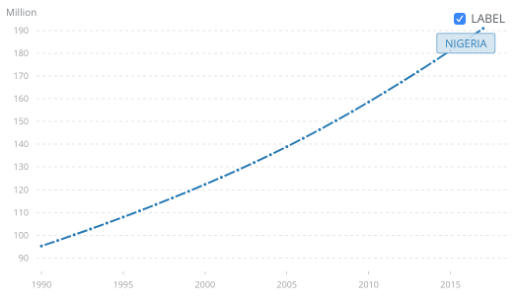
\includegraphics[width=8cm,height=4.5cm]{BF201-IMG/2.png}
        \end{center}

        \textbf{Figure 3: Population Pyramids}

        \begin{center}
                
\includegraphics[width=5cm,height=5cm]{BF201-IMG/3.png}
        \end{center}

	\newpage

	\textbf{Figure 4: Population of Sample Developed Country (UK)}

        \begin{center}
                
\includegraphics[width=8cm,height=4.5cm]{BF201-IMG/4.png}
        \end{center}

	\textbf{Figure 5: Fertility Rate in Sample Developed Country (UK)}

        \begin{center}
                
\includegraphics[width=8cm,height=4.5cm]{BF201-IMG/5.png}
        \end{center}

	\textbf{Figure 6: Average Earnings in Sample Developed Country (UK)}

        \begin{center}
                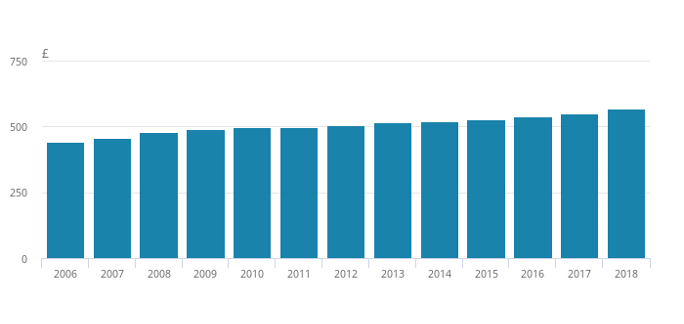
\includegraphics[width=10cm,height=4cm]{BF201-IMG/6.png}
        \end{center}

	\newpage

	\textbf{Figure 7: GDP of Sample Developed Country (UK)}

        \begin{center}
                
\includegraphics[width=8cm,height=4.5cm]{BF201-IMG/8.png}
        \end{center}

        \textbf{Figure 8: Global GDP}

        \begin{center}
                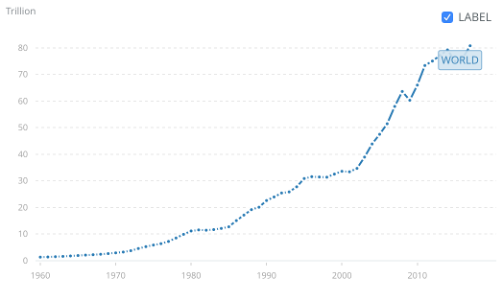
\includegraphics[width=8cm,height=4.5cm]{BF201-IMG/9.png}
        \end{center}

	\textbf{Model 1: Expansionary Monetary Policy}

	\begin{center}
		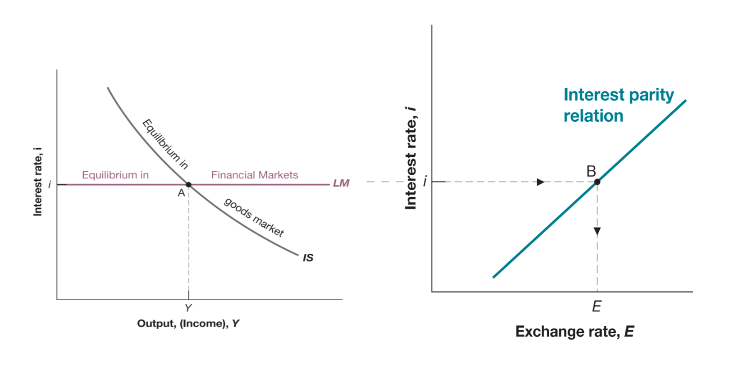
\includegraphics[width=9.5cm,height=5cm]{BF201-IMG/7.png}
	\end{center}

	Where: Expansionary Monetary Policy refers to in injection of money to the economy which leads to less money demanded, making currency less valuable and therefore lowering interest rate. This lowered interest rate shifts the Liquidity-Money (LM) curve down on the left graph which translates into a decrease in domestic exchange rate through the interest parity condition, seen on the right.

	\textbf{Formula 1: Output/GPD in an Open Economy}

	$$Y=C+I+G+(X-IM)$$

	Where:\\
	$C=f(Y-T)$\\
	$I=f(Y,i)$\\
	$X=f(Y^*,E)$\\
	$IM=f(Y,E)$\\

	Where:\\
	$Y$ = Domestic Output\\
	$Y^*$ = Foreign Output\\
	$T$ = Tax Rate\\
	$(Y-T)=Y_D$ = Disposable Output `Income'\\
	$i$ = Interest Rate\\
	$E$ = Nominal Domestic Exchange Rate\\
	$C$ = Consumption ($+$ Corr. w/ Disposable Income)\\
	$I$ = Investment ($+$ Corr. w/ Output; $-$ Corr. w/ Interest Rate)\\
	$G$ = Government Spending\\
	$X$ = Domestic Exports ($+$ Corr. w/ Foreign Income; $-$ Corr. w/ Nominal Domestic Exchange Rate)\\
	$IM$ = Domestic Imports ($+$ Corr. w/ Domestic Output; $+$ Corr. w/ Nominal Domestic Exchange Rate)\\

	Where:\\
	Output is a direct positive indicator of GDP\\
	``Output'' and ``Production'' can be used interchangeably\\

	\newpage

	\textbf{Formula 2: Wage Setting}

	$$\frac{W}{P^e}=(1-u)$$

	Where:\\
	$\frac{W}{P^e}$ = Real Expected Wage\\
	$W$ = Nominal Expected Wage\\
	$P^e$ = Expected Price of Goods Purchased\\
	$u$ = Unemployment ($+$ Corr. w/ Nominal Expected Wage; $-$ Corr. w/ Expected Price of Goods Purchased)

\newpage

	\renewcommand\refname{Bibliography}

	\begin{thebibliography}{9}

        \bibitem{a}
               	Altonji, J., Dunn, T. (1995).  
		\textsl{The Effects of School and Family Characteristics on the Return to Education.}
		Labor Studies.
			
	\bibitem{b}
                Aluko, OE. (2010).                                     
                \textsl{The Impact of Urbanisation on Housing Development: The Lagos Experience, Nigeria.}                                              
      		Ethiopian Journal of Environmental Studies and Management.
	
	\bibitem{c}
                Anriquez, G. (2008).
                \textsl{Rural Population Change in developing Countries: Lessons for Policymaking.}                                              
      		Springer Berlin Heidelberg.
	
        \bibitem{d}
                Bauer. (2001).
		\textsl{Demographic Change, Development and the Economic Status of Women in East Asia.}
		Stanford University Press.
			
	\bibitem{e}
                Blanchard O., Amighini A., Giavazzi F. (2018).
                \textsl{Macroeconomics: A European Perspective.}
      		Pearson Education Limited.
	
	\bibitem{f}
                Bongaarts, J. (2009).           
                \textsl{Human Population Growth and The Demographic Transition.}
     		Philosophical Transactions of the Royal Society of London. Series B: Biological Sciences. 

        \bibitem{g}
                Bullard, J., Keating, J. (1995).
		\textsl{The Long-Run Relationship Between Inflation and Output in Postwar Economies.}
		Journal of Monetary Economics. Elsevier Publishing.
			
	\bibitem{h}
                Chaparro, R., Kulkarni, K. (2015).
                \textsl{Does High Population Growth Help or Hurt Economic Development?.}
      		International Journal of Education Economics and Development.
	
	\bibitem{i}
                Gerald, M., Meier, G. (1995).
                \textsl{Leading Issues in Economic Development.}
     		Oxford University Press. 
	
	\bibitem{j}
                Goldin, C., Katz, F. (2002).             
                \textsl{The Power of the Pill: Oral Contraceptives and Women’s Career and Marriage Decisions.}                                            
      		Journal of Political Economy.

        \bibitem{k}
        	Goldin, C. (2006).        
		\textsl{The Quiet Revolution That Transformed Women’s Employment, Education and Family.}
		AEA Papers and Proceedings.
			
	\bibitem{l}
                Hunt, J., Friedberg, R. (1995).           
                \textsl{The Impact of Immigrants on Host Country Wages, Employment and Growth (In Symposia: Immigration).}                          
      		The Journal of Economic Perspectives.
	
	\bibitem{m}
                Lee, Ronald, Mason. (2011).
                \textsl{Population Aging and the Generational Economy: A Global Perspective..}                                             
      		Cheltenham, UK: Edward Elgar.
	
        \bibitem{n}
                Lee, R., Mason, A. (2013).
		\textsl{Population Change and Economic Growth in Africa.}
		National Transfer Accounts Publications.
			
	\bibitem{o}
                Levine, R. (1998).
                \textsl{The Legal Environment, Banks and Long-Run Economic Growth.}
		Journal of Money, Credit and Banking.
	
	\bibitem{p}
                Malthus, T. (1798).
                \textsl{An Essay on the Principal of Population.}
     		Cambridge University Press.

        \bibitem{q}
                Martin, P. (2009).
		\textsl{Demographic and Economic Trends: Implications for International Mobility.}
		United Nations Development Programme Human Development Reports.
			
	\bibitem{r}
                Mason, C. (2003).
                \textsl{Population Change and Economic Development.}                                        Open Mind Journals: University of Hawaii \& East-Coast Centre
	
	\bibitem{s}
        	National Transfer Accounts. (2013).
                \textsl{Data: Nigeria.} 
		National Transfer Accounts.
	
	\bibitem{t}
                Office for National Statistics (2017).          
                \textsl{Employee Earnings in the UK.}

        \bibitem{u}
                Office for National Statistics (2018).
		\textsl{Regional Labour Market Statistics in the UK: February 2019.}
			
	\bibitem{v}
                Republic of Kenya (2010).
                \textsl{2009 Kenya Population and Housing Census.}
		Government Printer Nairobi.
	
	\bibitem{w}
                Scott, J. (2009).           
                \textsl{Women and Employment: Changing Lives and New Challenges.}
     		Human Resource Management International Digest. Emerald Group Publishing Limited. 
	
        \bibitem{x}
                Singh, S., Darroch, J. (YYYY).
		\textsl{Adolescent Pregnancy and Childbearing: Levels and Trends in Developed Countries.}
		Family Planning Perspectives. Guttmacher Institute.
			
	\bibitem{y}
        	Thuku, G. (2013).
                \textsl{The Impact of Population Change on Economic Growth in Kenya.}                       International Journal of Economics \& Management Sciences. Katarina University.
	
	\bibitem{z}
                Van de Walle, F. (1986).
                \textsl{Infant Mortality and the European Demographic Transition.}
      		Princeton University Press.

        \bibitem{aa}
                World Bank. (2017).
		\textsl{GDP (Current \$).}
			
	\bibitem{ab}
                World Bank. (2017).           
                \textsl{Nigeria: Population, Total.}
	
	\bibitem{ac}
                World Bank. (2017).                  
                \textsl{United Kingdom: Fertility Rate, Total (Births Per Woman).}
	
	\bibitem{ad}
                World Bank. (2017).                  
                \textsl{United Kingdom: GDP (Current US\$).}
      
	\bibitem{ae}
                World Bank. (2017).                  
                \textsl{United Kingdom: Population, Total.}

	\end{thebibliography}

\end{document}
